\section{Auswertung}
\label{sec:Auswertung}

\subsection{Dichte der Kugeln}
\label{sec:DichtederKugel}
Die Messwerte der Massen und Radien der beiden Kugeln sind in Tabelle \ref{tab:MasseundDichte} zu finden.
Die Radien und Massen bestimmen sich zu
\begin{align*}
  r_{\symup{Gr}} &= (7,86 \pm 0,04)\cdot 10^{-3} \,\si{\meter}\\
  m_{\symup{Gr}} &= (4,54 \pm 0,01) \cdot 10^{-3} \,\si{\kilo\gram}\\
  r_{\symup{Kl}} &= (7,64 \pm 0,11)\cdot 10^{-3} \,\si{\meter}\\
  m_{\symup{Kl}} &= (4,44 \pm 0,02) \cdot 10^{-3} \,\si{\kilo\gram}.\\
\end{align*}

\begin{table}
  \centering
  \caption{Messdaten der Massen und Radien der beiden Kugeln.}
  \label{tab:MasseundDichte}
  \begin{tabular}{c c c c}
    \toprule
    $r_{\symup{Gr}}/\unit{\centi\meter}$ & $m_{\symup{Gr}}/\unit{\gram}$ & $r_{\symup{Kl}}/\unit{\centi\meter}$ & $m_{\symup{Kl}}/\unit{\gram}$ \\
    \midrule
    0,790 & 4,54 & 0,775 & 4,46 \\
    0,780 & 4,56 & 0,755 & 4,46 \\
    0,785 & 4,54 & 0,755 & 4,43 \\
    0,790 & 4,54 & 0,780 & 4,42 \\
    0,785 & 4,54 & 0,755 & 4,43 \\
    \bottomrule
  \end{tabular}
\end{table}

Aus () ergibt sich für die Dichten
\begin{align*}
  \rho_{\symup{Gr}} &= (2232 \pm 34) \,\frac{\si{\kg}}{\si{m^3}}  \\
  \rho_{\symup{Kl}} &= (2380 \pm 10) \,\frac{\si{\kg}}{\si{m^3}}. \\
\end{align*}

\subsection{Viskositätsbestimmung mit Hilfe der großen Kugel}
\label{ViskositaetGr}

\subsection{Viskositätsbestimmung mit Hilfe der kleinen Kugel}
\label{ViskositaetKl}

\subsection{Viskositäts}


\begin{figure}
  \centering
  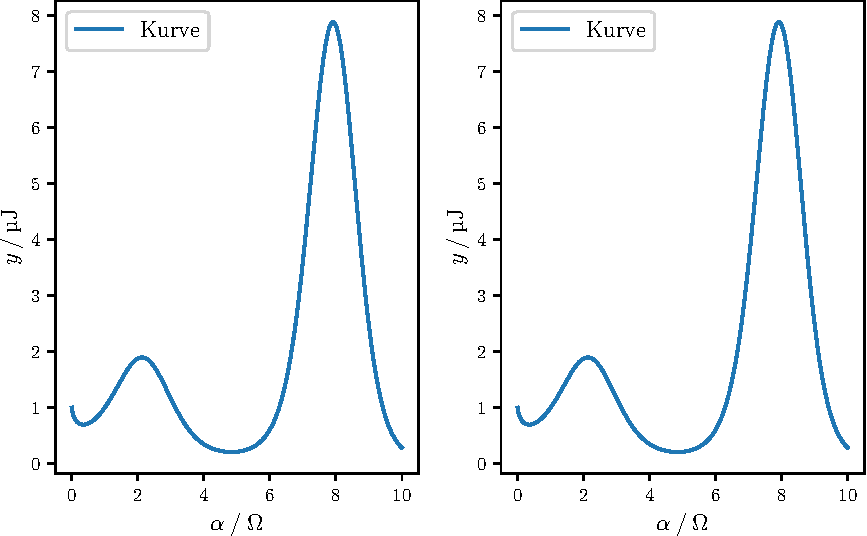
\includegraphics{plot.pdf}
  \caption{Plot.}
  \label{fig:plot}
\end{figure}


Siehe \autoref{fig:plot}!
